\documentclass{article}
\usepackage{fancyhdr} % Required for custom headers
\usepackage{lastpage} % Required to determine the last page for the footer
\usepackage{extramarks} % Required for headers and footers
\usepackage{graphicx} % Required to insert images
%\usepackage{lipsum} % Used for inserting dummy 'Lorem ipsum' text into the template
\usepackage{amsmath}
%\usepackage{amsfont}
%\usepackage{amssymb}

\usepackage{multicol}
% Margins
\topmargin=-0.5in
\evensidemargin=0in
\oddsidemargin=-0.5in
\textwidth=7.5in
\textheight=9.0in
\headsep=0.25in 


\pagestyle{fancy}

\rhead{M. Adam} % Top right header
\lhead{Pancakes}
\chead{ }
%\title{}

\begin{document}
%
%PRELIMINARIES:
%
%
%Begin by preheating the oven to 350 $^o$F
%
%\bigskip
%
%\bigskip

\begin{multicols}{2}
Ingredients:
\begin{itemize}
\item 2 bananas
\item 3 eggs
\item 1/4 cup almond oil
\item 1 tsp vanilla essence
\item 2/3 cup plain yogurt
\item 2 tbsp sugar
\item 1 3/4 cup gluten-free backing mix (with raising agent)
\item If using plain flour, add 1 tsp baking powder
\item 2 tbsp chia seeds (optional)
\item Butter for pan
\end{itemize}

\columnbreak

Directions:
\begin{enumerate}
\item While heating a flat pan on medium heat place all ingredients into a blender (wet ingredients first), and blend.

\item Melt a small amount of butter on the pan and pour out small circles of batter.

\item Cook on the first side until small bubbles appear, then flip and cook for an additional 1-2 minutes on the second side.
\end{enumerate}
\end{multicols}



\begin{center}
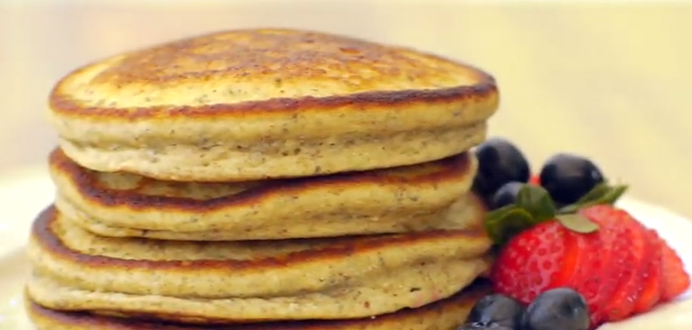
\includegraphics[scale=0.4]{Pancakes.png}
\end{center}


\end{document} 











